\documentclass[12pt, letterpaper]{article}

\usepackage{amsmath} % needed for including equations
\usepackage[margin=1in]{geometry} % sets the margins to 1in
\usepackage{graphicx} % needed for figures
\graphicspath{{./figures/}} % allows figures to be placed in a different folder
\usepackage[hang,small,bf]{caption} % sets the style on the figure captions
\usepackage{epstopdf} % converts eps files to pdf to display in the latex document



\begin{document}

\begin{titlepage}

\begin{center}

\vspace*{\fill}

\vspace{0.5in}

% Insert your title here
{ \LARGE \bfseries Collaborative Simultaneous UAV Exploration and Mapping In GPS Denied Environments Using a Relative Framework}\\[.25in]

\large
by\\[.25 in]
% Change your name here
Jacob M. Olson\\[1in]

A prospectus submitted to the faculty of\\
Department of Mechanical Engineering\\
Brigham Young University

\vspace{1in}

\today

\vspace*{\fill}

\end{center}

\end{titlepage}

\thispagestyle{empty}

\begin{center}
\vspace*{\fill}

\begin{figure}[htbp] %  figure placement: here, top, bottom, or page
   \centering
   
\includegraphics[width=2.5in]{byume_logo_clear.jpg} 
\end{figure}

\vspace{0.5in}

\Large{Prospectus Approval}\\[0.5in]

\end{center}

\hspace*{.47in}
\begin{minipage}[c]{5.25in}

\normalsize

Prospectus submitted by:

\vspace{.5in}

\makebox[2in]{\hrulefill} \hspace{1in} \makebox[2in]{\hrulefill}

% Change your name here
\parbox[b]{3in}{Your name} \, Date
\vspace{0.5in}

This prospectus has been approved by each member of the Graduate Committee:
\vspace{0.5in}

\makebox[2in]{\hrulefill} \hspace{1in} \makebox[2in]{\hrulefill}

\parbox[b]{3in}{Committee Member - Chair} \, Date
\vspace{0.4in}

\makebox[2in]{\hrulefill} \hspace{1in} \makebox[2in]{\hrulefill}

\parbox[b]{3in}{Committee Member} \, Date
\vspace{0.4in}

\makebox[2in]{\hrulefill} \hspace{1in} \makebox[2in]{\hrulefill}

\parbox[b]{3in}{Committee Member} \, Date

\end{minipage}

\vspace*{\fill}

\pagebreak

\setcounter{page}{1}

\section{Problem Statement}
After a disaster such as an earthquake or fire, buildings are often left structurally unsound. Sending in a human team to inspect the building can unnecessarily put human lives at risk. This project seeks to minimize the problem by sending in a swarm of intelligent unmanned aerial vehicles (UAVs), able to map a building, scan for damaged structures, and identify the source of a fire to determine the level of damage and whether or not it is safe to send in humans. 

Recent advances in GPS-denied navigation \cite{Wheeler2017} make it possible for UAVs to safely and accurately localize themselves in GPS degraded environments without colliding with obstacles, making indoor exploration and mapping possible. 

Because UAVs inherently have a very short battery life span, the optimization of search routes is imperative to their success in exploring and mapping an area. They must also be able to collaborate in their efforts to map and scan the building to quickly deliver results to a ground station. There are many mapping algorithms that work excellently with a single UAV, but collaborative, simultaneous mapping with UAVs is a not as developed. Leveraging multiple UAVs simultaneously mapping an area and meshing the data into a single map will greatly decrease the time it takes to survey and map an area. This will make it more feasible for UAVs to quickly survey a building in an emergency and get the information to first responders without risking human lives.

The objective of this proposed research is to develop a method that leverages multiple UAVs by optimally plans their search routes, and efficiently meshing data from the on-board sensors of the UAVs into a single, human-readable map. 

\begin{figure}[h] %  figure placement: here, top,  bottom, or page
   \centering
   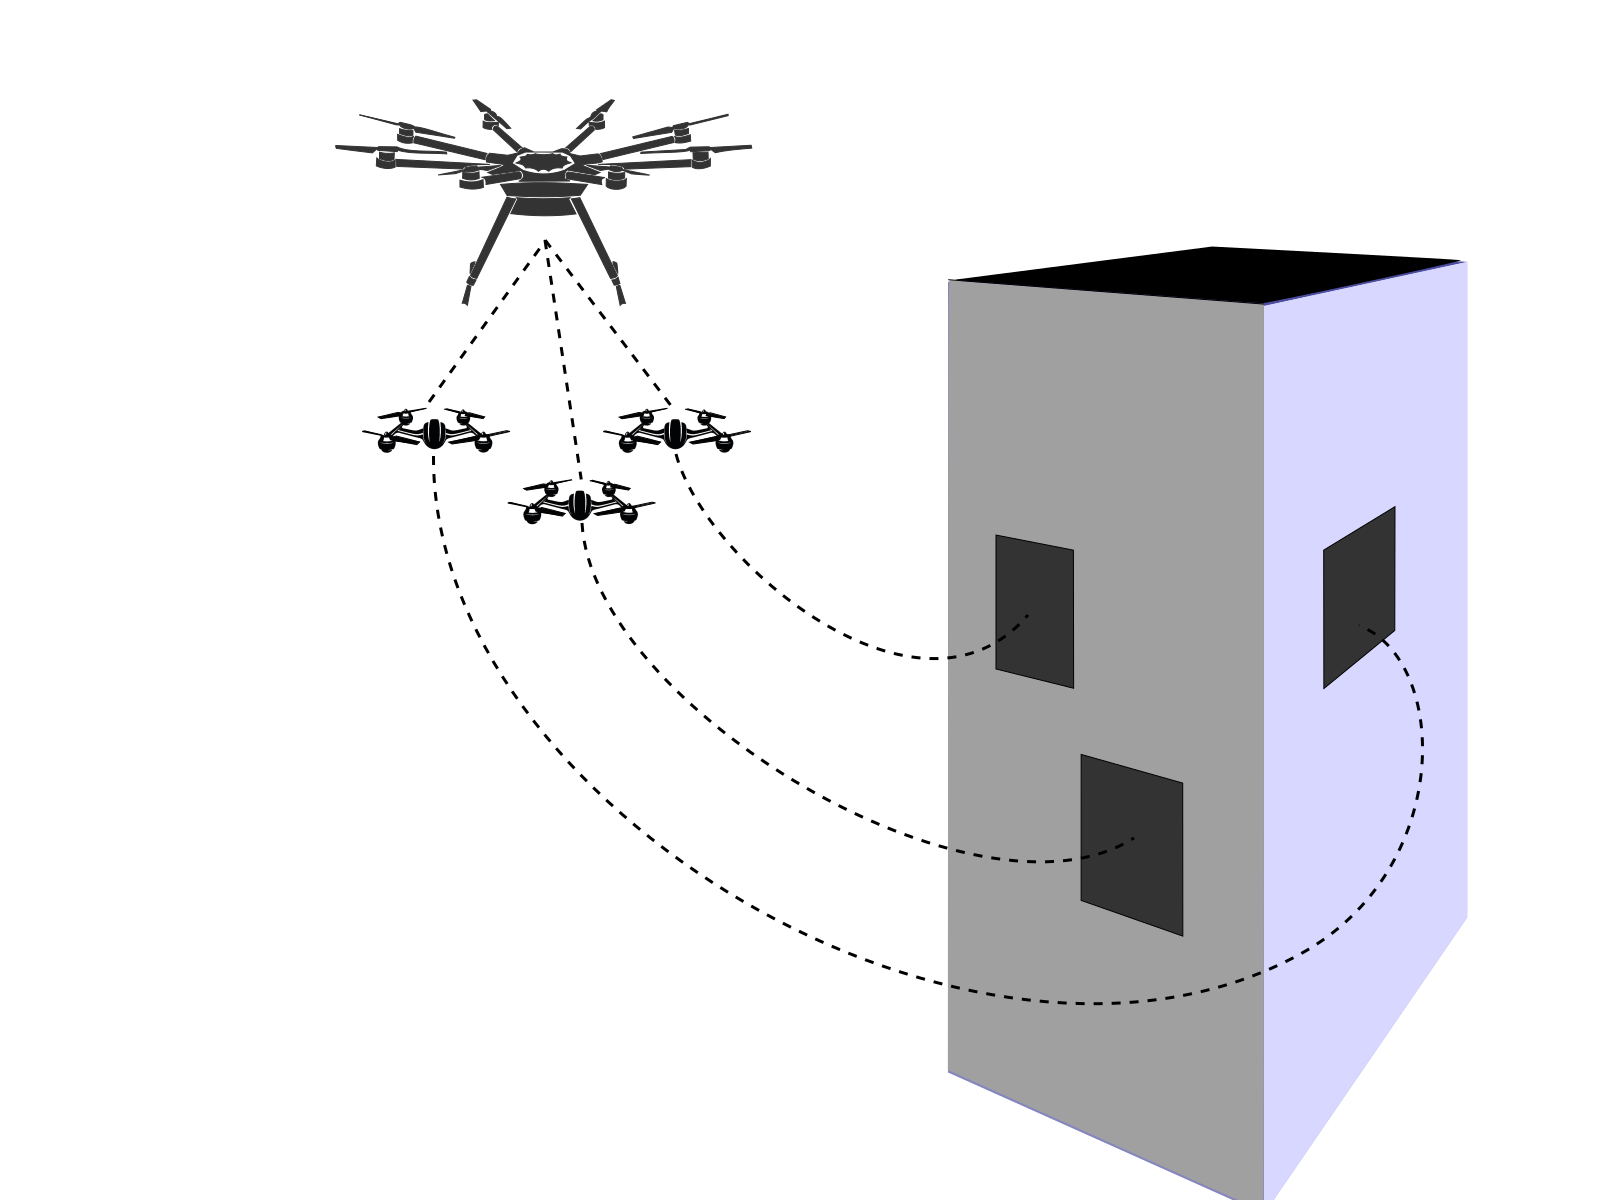
\includegraphics[trim = 0mm 0mm 0mm 0mm,clip,width=3in]{survey_drone_illustration.png}
   \caption{Survey UAVs deploy from Sentinel UAV to map a GPS-Denied area}
   \label{fig:sentinel_survey}
\end{figure}

\section{Background}

There are many approaches to the mapping problem for UAVs which can be split up into different categories

\subsection{Sensors} 
The sensors mounted on the UAVs greatly affect how they are able to map their environments. Monocualar cameras have been around the longest and are the most lightwieght, but are hardest to use in mapping a 3 dimensional environment. A newer technology that greatly increased the potential of 3D perception of cameras are stereo cameras. Made up of two cameras set up side by side, this type of camera allows for easier depth extraction from images. These cameras work much better than monocular cameras, but are still limited in their ability to reliably extract depth information from a camera. In the last several years, RGBD (RGB Depth) 3D cameras have emerged. these cameras are much better at reliably extracting depth information from the scene. Rather than just a stereo pair, RGBD cameras have a standard RGB (color) camera, a stereo pair of IR (Infrared) cameras, and an IR Projector, these all work together to produce a high resolution color image with an associatedd depth for each pixel in the image. These cameras have already had a significant impact on robotics and autonomy applications (Cite someting here). Until recently, however, these cameras have had a very large form factor compared to monocular and stereo cameras, making it hard for these cameras to be used on small UAVs. Intel, one of the industry leaders in RGBD camera technology, recently released a line of small lightweight, very capable RGBD cameras. The Intel RealSense D435 is the camera that will be used on this project.

Another type of sensor that should be noted is 3D and 2D scanning LiDAR sensors. Rather than return an image, these sensors are able to return a 360 degree representation of the environment. These sensors are very powerful, especially the 3D sensors, but as of writing this, due to the size of these sensors, it is infeasible to carry one on the size of UAV that will be used on this project. There are some smaller 2D scanning LiDAR sensors that are more feasible to use and one will likely be used for obstacle avoidance for this project.
 
\subsection{Data Structures} 
There are different approaches to the way mapping data is stored and used in mapping. 
Voxels - 3d pixels used for reconstructing and representing environment in 3D space. Either very data heavy or low resolution depending on size of them, limited area representation
Octomaps- Scale with detail, allow for more detail in detailed areas and less data usage in large open areas or closed areas \cite{Hornung2013}
Pointclouds- very dense, by default LiDAR and RGBD cameras return these, not ideal for 3D maps, but can be good for 2D ones


\subsection{Algorithms} (maybe combine this section with data structures)
SLAM - Simultaneous Localization and Mapping works well, better with few landmarks (is this the only way for this to work?)
Occupancy grid mapping- more dense, uses above items

\subsection{Planning}
In 2007 Bryson et. al. \cite{Bryson2007} demonstrated the ability to plan multiple flight paths and navigate an area using multiple UAVs flying concurrently using an EKF-SLAM Algorithm. This research was successful in having multiple agents find the same landmarks and create a single landmark map used to localize all UAVs. This research was done outdoors, not in a GPS Denied environment and it was a landmark-based EKF-SLAM so the resulting map is nothing more than landmark locations, making the map not very useful to for first responders. 
 
In 2012 Micheal et. al. \cite{Michael2012} tackled some of the collaborative mapping problem by using ground and aerial robots to collaboratively map an earthquake damaged building. They used a LiDAR scanner and an RGB-D camera and mapped the building using a voxel grid. They were able to successfully merge the maps into a single well structured map. Their results were lacking simultaneous mapping and a high enough resolution on their maps to be used effectively by search and rescue teams.   

From this brief survey of the current research, it can be seen that although various and significant contributions have been made in the field of collaborative planning and mapping, there is still great opportunity for continued research.  The research I would like to propose I believe would help to move some of the current research from the simulation and simplified use case, to real-world application.

\section{Research Objectives}

To successfully complete this proposed research, the following objectives will be accomplished:


\begin{itemize}

	\item Build up a simulation environment that models and controls generic quadrotor UAVs with appropriate sensors and an environment to be explored

	\item Develop (or implement) Optimal planning algorithm that determines the UAV flight path to successfully map full search area with loop closure to mesh maps  

	\item Determine and implement the best approach to mapping the area that will be human readable and provide sufficient information for action
	
	\item Develop a way for the UAVs to share map information so that the maps can be meshed together 

	\item Implement the solution in hardware on quadrotor UAVs to simultaneously explore and map a GPS denied environment
	
	\item Perform flight test demonstrations and gather test data to showcase the effectiveness of the solution that has been developed.

\end{itemize}

\section{Proposed Research}

To address the research, a multi-phase approach will be used. Research will commence by first setting up simulation environment in ROS Gazebo to allow for frequent testing without needing to rely on hardware every step of the way. Once the environment is set up, the project will be broken into three milestone hardware demonstrations: 

\subsection{Phase 1}
The first demonstration will be flying a single UAV in a GPS-denied environment to collect data and map the area. To complete this demonstration, an algorithm will need to be developed or implemented to plan the path in 3D space based off of a CAD model or blueprints of the search area. This path will be adjusted when unexpected obstacles and changes from the initial plans are detected. Although using a good odometry algorithm is essential to the success of this project, there are other students who are focusing on that aspect. 

Along with this phase, research will be done to determine the best mapping algorithm for this scenario. It will then be implemented on the UAV to map the environment. 

\subsection{Phase 2}
The second phase of the project will be to get a single UAV to fly multiple paths in the same environment. These paths will need to be optimized such that they cover the desired search area and overlap enough to provide sufficient loop closure to mesh the maps together in post processing. This is where the bulk of the unique research will be done. As mentioned earlier, there has not been significant research done in the area of meshing maps from multiple UAVs into a single map. 

\subsection{Phase 3}
The third and final phase of the project will be to get multiple UAVs flying simultaneously in the same environment and meshing the maps of them into a single map. This will require more effort on the path planning to make sure the paths can be flown simultaneously, then something clever will be done to make the map meshing as close to real time as possible. 

\begin{figure}[t] %  figure placement: here, top,  bottom, or page
   \centering
   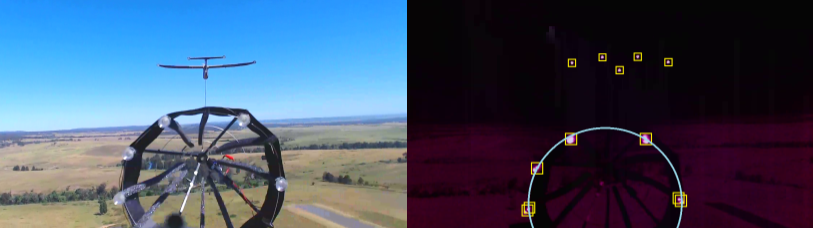
\includegraphics[trim = 0mm 0mm 0mm 0mm,clip,width=6in]{ir_drogue.png}
   \caption{Infrared markers as seen through RGB and IR cameras \cite{WilsonDB.2015}.}
   \label{fig:irmarkers}
\end{figure}

Brigham Young University, and specifically the MAGICC Lab, has a strong background in the field of Relative Navigation for UAS \cite{Leishman2013}.  Though the shipboard landing problem is significantly different than the relative navigation work that has been previously performed here, successful shipboard landing requires a form of relative navigation, and can likely draw on some of the relative navigation work that has already been done.  In the current relative navigation problem, measurements between the static surroundings and the dynamic UAS are taken to estimate the relative position and velocities of the UAS.  If we now flip the problem by assuming that the UAS is pseudo-stationary (i.e. its movement is small and its position is known thanks to GPS), we would like to explore the possibility of taking similar measurements to estimate the state of the dynamic surrounding (i.e. the ship deck). In the current relative navigation problem, an accurate estimate of the UAS' state is aided significantly by measurements from an on-board IMU. Similarly, we would like to research the contribution that a ship-based IMU can offer to enable a more robust shipboard landing solution.

Though much of this proposed research will begin in simulation, the resultant methods and solutions that are discovered are planned to be implemented in hardware flight tests.  Testing in hardware will require a quadrotor UAS to be procured and assembled, and will also require a ship deck motion emulator to be fabricated.  The UAS will be comprised of standard hobbyist equipment for the airframe and propulsion system, and the ship deck emulator will similarly be fabricated using off-the-shelf components.  Autopilot capabilities for the UAS will be enabled through the use of a ROSflight flight controller paired with an on-board computer that will run the autopilot control loops in Robot Operating System (ROS).  The ship deck emulator is planned to have its own GPS receiver and IMU unit.  Communication of sensor measurements and/or state estimates from the ship deck emulator to the UAS are planned to be communicated over a local WiFi network.  At all times during flight test operations the UAS will be controllable through a ground-station computer, and a safety pilot will be present to take manual control of the UAS at any moment.  When satisfactory results from flight demonstrations are obtained, the data will be collected, analyzed, and presented in the form of a formal Thesis. 



%The experimental apparatus will have instrumentation to measure pressures, temperatures, and mass flow.
%The pressures and temperatures will be measured at the turbine and compressor inlets and outlets. Pressures will be measured using pressure transducers and temperatures using thermocouples. The thrust will be measured using an air bearing system to decrease friction and a strain gauge. The mass flow into the compressor and turbine will be measured.
%Turbine power will be measured using the compressor work. Exact power measurement is not necessary since a comparison will be made on the same equipment and not with independently collected data.

%Experimental data will be used to compare steady and pulsed flow. Comparisons will be made using specific power, turbine efficiency, and a turbine map. Specific thrust and power will both be calculated by dividing the respective quantities by the mass flow rate through the turbine. The conventional methods used to calculate turbine efficiency are not adequate due to the unsteady flow conditions. A method to include the unsteady effects in the calculation of efficiency is still being investigated.

%An example of an equation is shown in Equation~\ref{eq:efficiency}.

%\begin{equation}
%\eta_t = \cfrac{\dot W_c + \dot W_{fric}}{\dot m c_p \left[ 1 - \left( \cfrac{p_{t5}}{p_{t4}} \right)^\frac{\gamma - 1}{\gamma} \right]}
%\label{eq:efficiency}
%\end{equation}

%Flack \cite{flack:2008fundamentals-of} presents a method to create a turbine map. Both turbine pressure ratio and efficiency can be expressed as functions of corrected mass flow and rotational speed as shown in Equations~\ref{pressure_ratio} and~\ref{efficiency_function}.
%
%\begin{equation}
%\frac{p_{t4}}{p_{t5}} = \mathscr{F} \left\{ \frac{\dot m \sqrt{\theta_{t4}}}{\delta_{t4}}, \frac{N}{\sqrt{\theta_{t4}}} \right\} = \mathscr{F} \left\{ \dot m_{c4}, N_{c4} \right\}
%\label{pressure_ratio}
%\end{equation}
%%
%\begin{equation}
%\eta = \mathscr{G} \left\{ \frac{\dot m \sqrt{\theta_{t4}}}{\delta_{t4}} , \frac{N}{\sqrt{\theta_{t4}}} \right\} = \mathscr{G} \left\{ \dot m_{c4}, N_{c4} \right\}
%\label{efficiency_function}
%\end{equation}
%%
%where
%\[\delta_{t4} = p_{t4}/p_{stp}\]
%and
%\[\theta_{t4} = T_{t4}/T_{stp}\]
%%
%Lines of constant corrected speed and efficiency will then be plotted on an axis of pressure ratio versus corrected mass flow.

\section{Anticipated Contributions}

As a result of this research, there will be an improved understanding of how robust maritime landing can be achieved for real-world applications and conditions.  Specifically, it is anticipated that this work will demonstrate the contributions that an IR vision system and shipboard IMU can make in helping to ensure a soft and safe landing. Although there are many shipboard landing methods that have already been developed, this proposed research seeks to extend and add to current methods to a degree that is new and unique.  Maritime landing in darkness, and landing with ship deck IMU data, are both areas that appear to be absent in the current literature. Good results coming out of this research would open opportunities for possible journal or conference paper publications, and would also pave the way to further research opportunities for future students.    

%  A direct comparison will be made between a steady and unsteady flow through an axial turbine without any bypass flow. This direct comparison has not been previously performed. Possible publications from this research include presenting at the ASME Turbo Expo, submitting to the ASME Journal of Turbomachinery, presenting at the AIAA Aerospace Science Meeting, or other conferences and journals. This research is sponsored by Innovative Scientific Solutions, Inc. through an Air Force contract.

\pagebreak

\bibliographystyle{IEEEtran}
\bibliography{library}

\end{document}